The Poisson distribution is a discrete random distribution that can 
be used as an approximation of the Binomial distribution in cases where 
$n$ tends towards infinity and $r$ tends towards $0$ such that their 
product stays about equal to a parameter $\lambda$, which is the 
parameter of the Poisson distribution and also its expected value and 
variance. The outcome space of a Poisson random variable is 
$\mathbb{N}_0$, that is natural numbers including $0$, and its pmf,
expected value and variance are given by

$$
\begin{aligned}
    p(x) = \operatorname{Poisson}(x; \lambda) &= \frac{\lambda^x e^{-\lambda}}{x !}, \\
    E[X] = \operatorname{Var}[X] &= \lambda.
\end{aligned}
$$

The probability mass function and the corresponding cumulative density functions
of the Poisson distribution can be seen in Figure \ref{fig:poisson}.
The Poisson distribution is a critical component of modern multi-object
tracking systems, as it is used to model noise measurements, and some 
systems even use it to model objects that exist but are not visible in
the field of view of a sensor \cite{garcia-fernandezPoissonMultiBernoulliMixture2018}.
The Poisson distribution is the foundation of the so-called Poisson Point
Processes (PPP), which will be discussed later.

\begin{figure}
\centering
\begin{subfigure}{.5\textwidth}
  \centering
  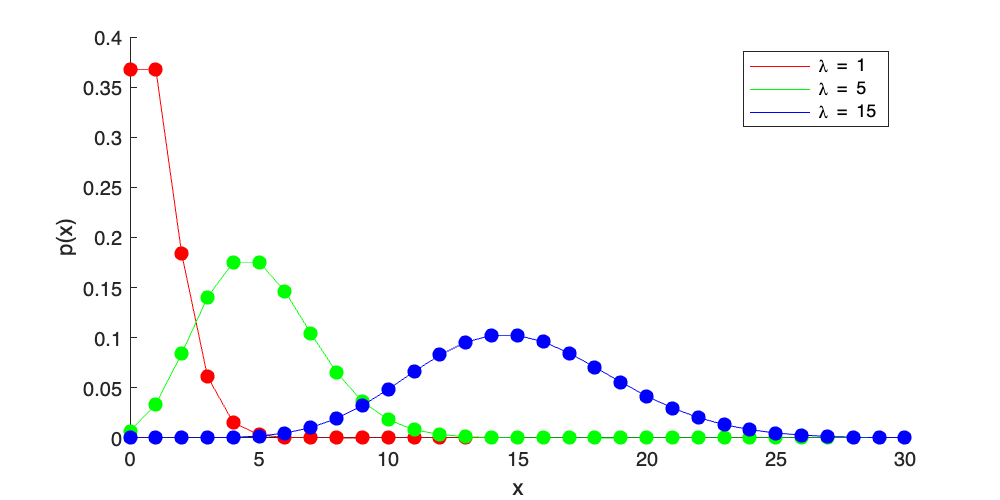
\includegraphics[width=.9\linewidth]{figures/poisson.pmf.png}
  \caption{PMF.}
  \label{fig:poisson:pmf}
\end{subfigure}\hfill
\begin{subfigure}{.5\textwidth}
  \centering
  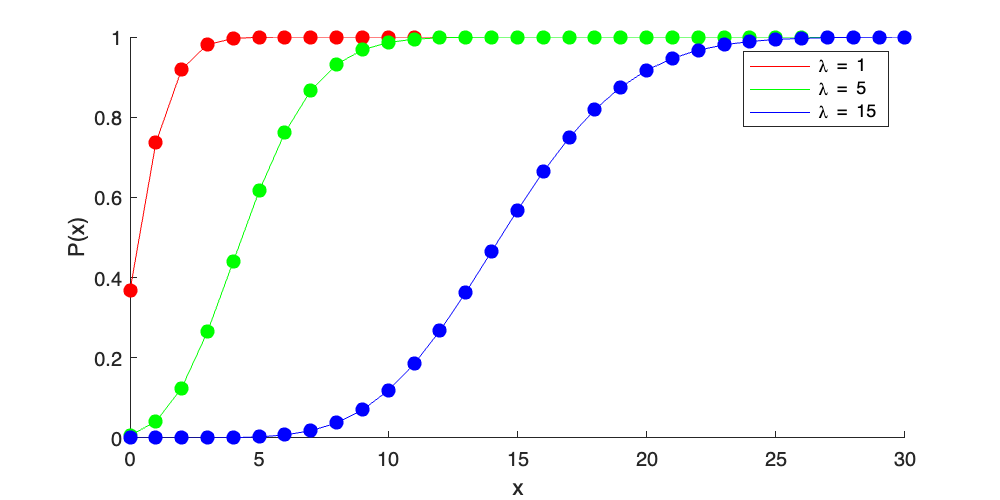
\includegraphics[width=.9\linewidth]{figures/poisson.cdf.png}
  \caption{CDF.}
  \label{fig:poisson:cdf}
\end{subfigure}
\caption{Poisson distribution.}
\label{fig:poisson}
\end{figure}
